In Kapitel 3 werden wir sehen, dass es möglich ist die Elementsteifigkeitsmatrix der Masse Matrix und der Laplace Bilinearform als einen Tensor umzudefinieren. Nachdem wir dies gemacht haben, werden wir die Strukturen dieses Tensors untersuchen, mit Hinblick einen einfachen Weg zu finden, die Pseudoinverse zu bestimmen. Was genau ein Tensor ist, was wir unter der Pseudoinversen eines Tensors verstehen und wie wir einen Tensor analyisieren, wird in diesem Unterkapitel beantwortet.


\begin{Definition} (Tensor) \\
Ein Tensor ist eine multidimensionale Matrix $\pmb{\mathscr{X}}  \in \mathbb{R}^{I_1 \times I_2 \times \dots \times I_N}$.
Die Ordnung ist die Anzahl der Dimensionen, in diesem Fall $N$.
\end{Definition}

\begin{figure}[ht]
	\centering
  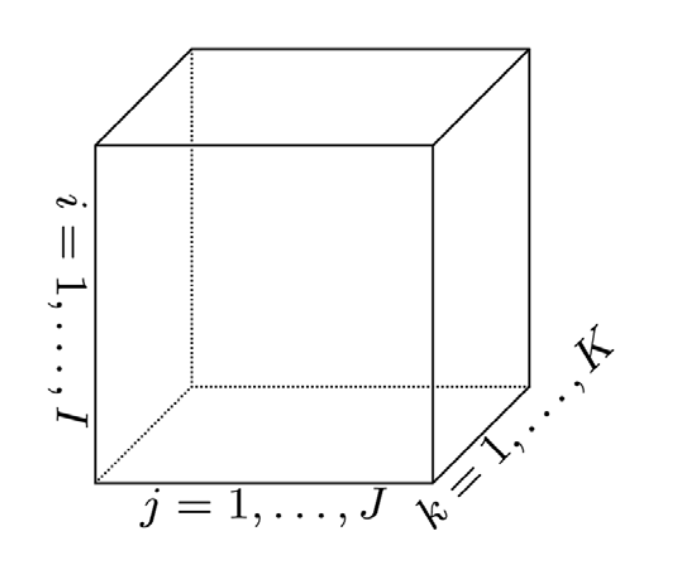
\includegraphics[width=0.3\textwidth]{tensorOrdnung3.png}
	\caption{Tensor 3.Ordnung $\pmb{\mathscr{X}}  \in \mathbb{R}^{I \times J \times K}$} \cite[456]{Kolda}
	\label{fig:tensorOrdnung3}
\end{figure}

Vorsicht zu haben, gilt es bei den Begriffen Ordnung und Rang bei Tensoren. Außerdem sollte man nicht den Begriff des Rangs einer Matrix, mit dem Begriff des Ranges eines Tensors verwechseln. 


\begin{Bemerkung} Symmetrie \\
\begin{itemize}
\item Ein Tensor nennt man kubisch genau dann wenn jeder Mode dieselbe Dimension hat. 
\item Einen kubischen Tensor nennt man supersymmetrisch genau dann wenn die Elemente des Tensors konstant bleiben unter jeglicher Permutation der Indizes
\item Ein Tensor kann stückweise symmetrisch sein wenn die Elemente konstant bleiben unter der Permutation von mindestens 2 Indizes.
\end{itemize}
\end{Bemerkung}

\begin{Definition} Diagonal \\
Einen Tensor ${\cal X}  \in \mathbb{R}^{I_1 \times I_2 \times \dots \times I_N}$ nennt man diagonal, wenn
$x_{i_1,\dots,i_N} \neq 0$ genau dann wenn $i_1 = \dots = i_N$.
\end{Definition}

\begin{Definition} Faser \\
Eine Faser ist das multidimensionale Analog zu Matrixspalten und Matrixzeilen. Wir definieren eine Faser, indem wir jeden Index abgesehen von einem festhalten.
\end{Definition}

\begin{Bemerkung} Entfaltung \\
Einen Tensor kann man entfalten. Dies impliziert eine neu ordnung der Tensorelemente in eine Matrix.
Wir betrachten nur die sogenannte Ordnung-n Entfaltung, da dies die einzig relevante Form der Entfaltung ist.
Eine Ordnung-n Entfaltung eines Tensors ${\cal X}  \in \mathbb{R}^{I_1 \times I_2 \times \dots \times I_N}$ wird mit $\bold{X}_{(n)}$ geschrieben und ordnet die Ordnung-n Fasern in die Spalten der Ergebnismatrix.
Formal ist es eine Abbildung des Indize N-tupels $(i_1,\dots,i_N)$ auf Matrixindizes $(i_n,j) $
\begin{equation}
j=1+\sum_{\substack{k=1 \\ k \neq n}}^{N} (i_k-1)J_k \text{ mit } J_k = \prod_{\substack{m=1 \\ m \neq n}}^{k-1} I_m
\end{equation}
\end{Bemerkung}

Nun fehlt uns noch eine Tensor Multiplikation um mit der Dekomposition von Tensoren anzufangen. 

\begin{Definition} n-Ordnung Produkt \\
Das n-Ordnung Produkt eiens Tensors  ${\cal X}  \in \mathbb{R}^{I_1 \times I_2 \times \dots \times I_N}$ mit einer Matrix $U \in \mathbb{R}^{J \times I_n}$ wird geschrieben als ${\cal X} \times_n U$ und die Ergebnis Matrix hat die Größe $I_1 \times \dots I_{n-1} \times J \times I_{n+1} \times \dots I_N$
\begin{equation}
	({\cal X} \times_n U)_{i_1 \dots i_{n-1} j i_{n+1} \dots i_N} = \sum_{i_n = 1}^{I_n} x_{i_1 \dots i_N} u_{j i_n}
\end{equation}
\end{Definition}

\begin{Bemerkung}
Jedes n-Ordnung Produkt kann mit Hilfe von entfaltenen Tensoren äquivalent ausgedrückt werden.
\begin{equation}
{\cal Y} = {\cal X} \times_n U \Longleftrightarrow Y_{(n)} = UX_{(n)}
\end{equation}
\end{Bemerkung}

\subsubsection{Singulärwertzerlegung höherer Ordnung}

Die Higher Order Singular Value Decomposition oder auch bekannt unter Tucker Decomposition ist eine uminterpretierte multidimensionale Hauptkomponentenanalyse. Man versucht durch Hauptachsentransformationen die Korrelation zwischen den verschiedenen Merkmalen durch Überführung in eine neue Basis zu minimieren. Die Hauptachsentransformation lässt sich durch eine orthogonale Matrix angeben, die aus den Eigenvektoren der Kovarianzmatrix gebildet wird. (Wikipedia: Hauptkomponentenanalyse).

Die HOSVD zerlegt den Tensor in einen Kern-Tensor (Core Tensor) multipliziert mit einer Matrix in jeder Ordnung. 

\begin{Beispiel} HOSVD Tensor 3.Ordnung
${\cal X}  \in \mathbb{R}^{I \times J \times K}$
\begin{equation}
{\cal X} \approx {\cal G} \times_1 A \times_2 B \times_3 C 
\end{equation}
Wobei $A \in \mathbb{R}^{I \times P}$, $B \in \mathbb{R}^{J \times Q}$ und $C \in \mathbb{R}^{K \times R}$ die Faktormatrizen sind, welche orthogonal sind.
${\cal G}$ bezeichnet den Kern-Tensor und zeigt wie hoch die Korrelation zwischen den verschiedenen Komponenten ist.
\end{Beispiel}

\begin{figure}[ht]
	\centering
  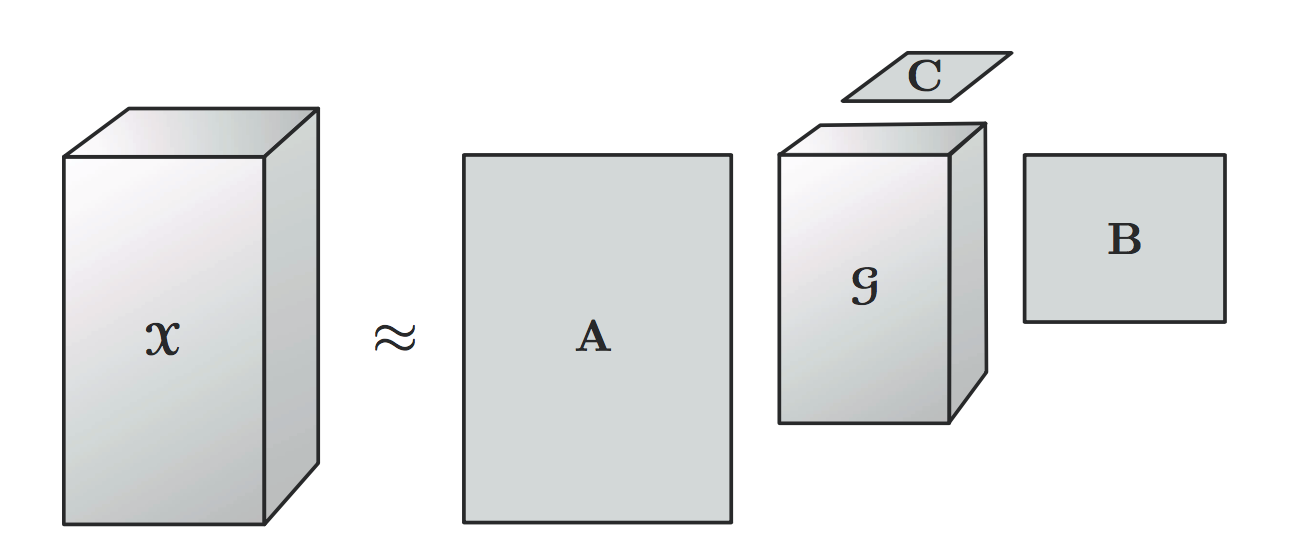
\includegraphics[width=0.6\textwidth]{hosvdTensor.png}
	\caption{HOSVD eines Tensors 3.Ordnung}
	\label{fig:hosvdTensor}
\end{figure}

\begin{Bemerkung} Entfaltete HOSVD \\
\begin{equation}
X_{(n)} = A^{(n)} G_{(n)} ( A^{(N)} \otimes \dots \otimes A^{(n+1)} \otimes A^{(n-1)} \otimes \dots \otimes A^{(1)} )^{T}
\end{equation}
\end{Bemerkung}


\begin{Bemerkung} Berechnung der HOSVD (Wikipedia) \\
Die Berechnung der HOSVD von ${\cal X}  \in \mathbb{R}^{I_1 \times I_2 \times \dots \times I_N}$ geht wie folgt
\begin{enumerate}
\item Berechne die Ordnung-k Entfaltungen ${\cal X}_{(k)}$ für alle k
\item Berechne die SVD ${\cal X}_{(k)}=U_k \Sigma_k V_k^T$ und speichere $U_k$
\item Der Kerntensor ${\cal S}$ ergibt sich aus der Projektion des Tensors auf die Tensorbasis geformt von den Faktormatrizen  $\{ U_k\}_{k=1}^{N}$  also ${\cal S}={\cal X} \times_{n=1}^{N} U_n^T$
\end{enumerate}
\end{Bemerkung}

\begin{Bemerkung} Eindeutigkeit der HOSVD \\
Die HOSVD ist keine eindeutige Zerlegung. Dies führen wir an einem Tensor 3.Ordnung an. Sei $U \in \mathbb{R}^{P \times P}$, $V \in \mathbb{R}^{Q \times Q}$  und $W \in \mathbb{R}^{R \times R}$ . Dann folgt
\begin{equation}
{\cal X} = {\cal G} \times_1 A \times_2 B \times_3 C = ({\cal G} \times_1 U \times_2 V \times_3 W) \times_1 AU^{-1} \times_2 BV^{-1} \times_3 CW^{-1}
\end{equation}
In anderen Worten: Wir können den Kerntensor ${\cal G}$ modifizieren ohne die Gleichung zu ändern, solange wir das Inverse der Modifizierung auf den zugehörigen Faktormatrizen multiplizieren.
\end{Bemerkung}

Mit diesen Kenntnissen können wir nun zum Beispiel versuchen soviele Elemente des Kerntensor wie möglich auf 0 zu bekommen oder so klein wie möglich zu machen.
Weiterführende Liteartur S.479 TENSOR DECOMPOSITIONS AND APPLICATIONS.

Wir brauchen noch einige Eigenschaften zum Kronecker Produkt, die wir uns später für die Berechnung der Pseudoinversen zu Nutze machen wollen.

\begin{Lemma}
Sind A,B invertierbar so ist auch $(A \otimes B)$ invertierbar. Mit der Inversen
\begin{equation*}
(A \otimes B)^{-1} = A^{-1} \otimes B^{-1}
\end{equation*}
Für die Moore Penrose Pseudoinversen gilt:
\begin{equation*}
(A \otimes B)^{+} = A^{+} \otimes B^{+}
\end{equation*}
\end{Lemma}

